\documentclass[a0paper,portrait]{article}
\usepackage[margin=2cm]{geometry}
\usepackage{graphicx}
\graphicspath{{images/}}
\usepackage{amsmath}
\usepackage{amssymb}
\usepackage{booktabs}
\usepackage{tikz}
\usetikzlibrary{shapes,arrows,positioning}
\usepackage{xcolor}
\usepackage{multicol}
\usepackage{listings}
\usepackage{calc}
\usepackage{url}
\usepackage{times}
\usepackage{enumitem}

% Define colors
\definecolor{headercol}{RGB}{70,40,160}
\definecolor{boxcolor}{RGB}{240,240,250}

\setlist[itemize]{leftmargin=*,nosep}

% Save space in lists
\newcommand{\compresslist}{%
\setlength{\itemsep}{0pt}%
\setlength{\parskip}{0pt}%
\setlength{\parsep}{0pt}%
}

% Define code style
\lstset{
    language=Python,
    basicstyle=\ttfamily\normalsize,
    keywordstyle=\color{blue},
    stringstyle=\color{red},
    commentstyle=\color{green!60!black},
    breaklines=true,
    showstringspaces=false,
    frame=single,
    backgroundcolor=\color{boxcolor}
}

% Custom section style
\usepackage{titlesec}
\titleformat{\section}
{\normalfont\huge\bfseries\color{headercol}}
{\thesection}{1em}{}

\begin{document}

\begin{center}
\textcolor{headercol}{\fontsize{40}{48}\selectfont\textbf{SnapML:}} \fontsize{40}{48}\selectfont\textbf{A Visual Programming Tool for Machine Learning}

\vspace{0.5cm}
{\LARGE A Block-Based Drag-and-Drop Interface for Machine Learning Development}

\vspace{1cm}
\begin{tabular}{c}
    \textbf{CS5351 Software Engineering Final Project | Team 8}\\
    \vspace{0.5cm}\\
    \textbf{Team Leader:} LI ZHIYU \\
    \textbf{Members:} CHANG CHONGYU, CHEN DATANG, FENG ZIXIAO, LI GUOQIONG, SUN CHENGWEI, YE KAI, ZONG WEIHANG
\end{tabular}
\end{center}

\begin{multicols}{2}

\section{Project Overview and Contributions}

\begin{center}
\includegraphics[width=0.9\linewidth]{程序界面.png}
\end{center}

SnapML is a drag-and-drop, block-based machine learning tool that enables developers to apply machine learning techniques more efficiently. It transforms the traditional coding process into an intuitive visual interface, similar to building with Lego blocks.

\textbf{\color{headercol}Key Contributions:}
\begin{itemize}\compresslist
    \item Lowered the technical barrier of ML development through visual abstraction of complex concepts
    \item Provided pre-built blocks for common machine learning tasks
    \item Simplified algorithm selection and configuration with guided model selection
    \item Implemented drag-and-drop data transformation to simplify data preprocessing
    \item Offered a streamlined workflow from data to deployment
\end{itemize}

By providing a visual approach to machine learning development, SnapML addresses the steep learning curve typically associated with ML, making it accessible to a broader audience including:
\begin{itemize}\compresslist
    \item Software developers without ML expertise
    \item Data scientists seeking rapid prototyping
    \item Educators teaching ML concepts
    \item Cross-functional teams with varying technical backgrounds
\end{itemize}

\section{Background \& Motivation}

With the rapid development of Machine Learning (ML), it has become an essential part of modern technology. However, many developers face significant barriers when attempting to implement ML solutions:

\begin{minipage}{0.5\linewidth}
\begin{center}
\begin{tabular}{|p{0.45\linewidth}|p{0.45\linewidth}|}
\hline
\textbf{Challenges} & \textbf{SnapML Solutions} \\
\hline
Complex mathematical theories & Visual abstraction of complex concepts \\
\hline
Extensive programming requirements & Pre-built blocks for common ML tasks \\
\hline
Algorithm selection difficulties & Guided model selection and configuration \\
\hline
Data preprocessing complexity & Drag-and-drop data transformation \\
\hline
Integration challenges & Streamlined workflow from data to deployment \\
\hline
\end{tabular}
\end{center}
\end{minipage}
\begin{minipage}{0.48\linewidth}
\includegraphics[width=\linewidth]{加载范例程序.png}
\end{minipage}

The need for a visual programming environment for ML arises from the growing demand for:
\begin{itemize}\compresslist
    \item Faster development cycles in data science projects
    \item Tools that facilitate learning and experimentation
    \item Accessible ML development for non-specialists
    \item Improved collaboration between technical and non-technical team members
\end{itemize}

\section{Technology Stack}

SnapML integrates several proven technologies to create a seamless machine learning development experience:

\begin{center}
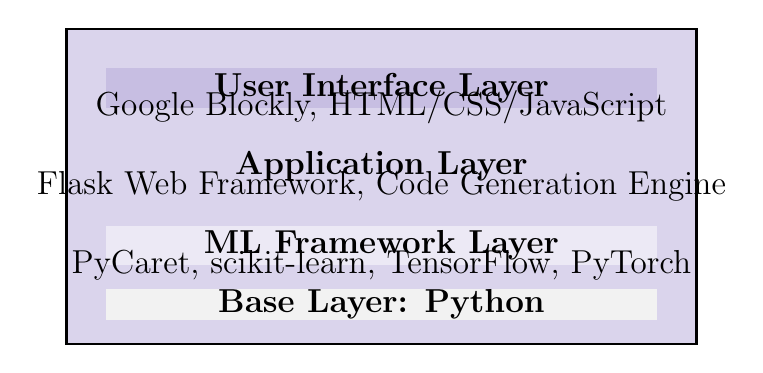
\begin{tikzpicture}
\fill[headercol!20] (0,0) rectangle (8,4);
\draw[thick] (0,0) rectangle (8,4);

% User Interface Layer
\fill[headercol!30] (0.5,3.0) rectangle (7.5,3.5);
\node[align=center] at (4,3.25) {\large \textbf{User Interface Layer}};
\node[align=center] at (4,3.0) {\large Google Blockly, HTML/CSS/JavaScript};

% Business Logic Layer
\fill[headercol!20] (0.5,2.0) rectangle (7.5,2.5);
\node[align=center] at (4,2.25) {\large \textbf{Application Layer}};
\node[align=center] at (4,2.0) {\large Flask Web Framework, Code Generation Engine};

% ML Framework Layer
\fill[headercol!10] (0.5,1.0) rectangle (7.5,1.5);
\node[align=center] at (4,1.25) {\large \textbf{ML Framework Layer}};
\node[align=center] at (4,1.0) {\large PyCaret, scikit-learn, TensorFlow, PyTorch};

% Base Layer
\fill[gray!10] (0.5,0.3) rectangle (7.5,0.7);
\node[align=center] at (4,0.5) {\large \textbf{Base Layer: Python}};
\end{tikzpicture}
\end{center}

\textbf{Key Technologies:}
\begin{itemize}\compresslist
    \item \textbf{Google Blockly:} Open-source visual programming library that forms the foundation of our drag-and-drop interface
    \item \textbf{Flask:} Lightweight Python Web framework for serving the application
    \item \textbf{PyCaret:} Low-code ML library that powers many of the built-in models
    \item \textbf{Python:} The underlying programming language that executes the generated code
\end{itemize}

\section{System Architecture}

SnapML follows a modular architecture designed for extensibility and ease of use:

\begin{center}
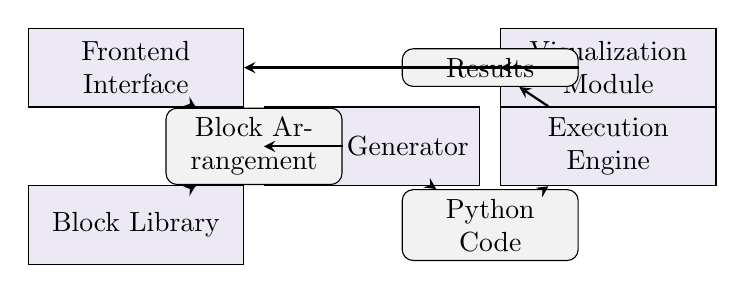
\begin{tikzpicture}
% Modules - using rectangles instead of custom shapes
\node[rectangle,draw,fill=headercol!10,text width=2.5cm,align=center,minimum height=1cm] (frontend) at (0,0) {Frontend Interface};
\node[rectangle,draw,fill=headercol!10,text width=2.5cm,align=center,minimum height=1cm] (blocklibrary) at (0,-2) {Block Library};
\node[rectangle,draw,fill=headercol!10,text width=2.5cm,align=center,minimum height=1cm] (codegen) at (3,-1) {Code Generator};
\node[rectangle,draw,fill=headercol!10,text width=2.5cm,align=center,minimum height=1cm] (execution) at (6,-1) {Execution Engine};
\node[rectangle,draw,fill=headercol!10,text width=2.5cm,align=center,minimum height=1cm] (viz) at (6,0) {Visualization Module};

% Data nodes - using rectangles with rounded corners
\node[rectangle,rounded corners,draw,fill=gray!10,text width=2cm,align=center] (blocks) at (1.5,-1) {Block Arrangement};
\node[rectangle,rounded corners,draw,fill=gray!10,text width=2cm,align=center] (code) at (4.5,-2) {Python Code};
\node[rectangle,rounded corners,draw,fill=gray!10,text width=2cm,align=center] (results) at (4.5,0) {Results};

% Arrows
\draw[->,>=stealth,thick] (frontend) -- (blocks);
\draw[->,>=stealth,thick] (blocklibrary) -- (blocks);
\draw[->,>=stealth,thick] (blocks) -- (codegen);
\draw[->,>=stealth,thick] (codegen) -- (code);
\draw[->,>=stealth,thick] (code) -- (execution);
\draw[->,>=stealth,thick] (execution) -- (results);
\draw[->,>=stealth,thick] (results) -- (viz);
\draw[->,>=stealth,thick] (viz) -- (frontend);

\end{tikzpicture}
\end{center}

\textbf{Components:}
\begin{description}
    \item[Frontend Interface:] Provides the block workspace, preview panel, and settings controls
    \item[Block Library:] Contains all available ML-specific blocks organized by category
    \item[Code Generator:] Translates the visual block arrangement into executable Python code
    \item[Execution Engine:] Runs the generated code on the server and handles data processing
    \item[Visualization Module:] Renders results in various formats (charts, tables, metrics)
\end{description}

The data flow follows a clear path:
\begin{enumerate}\compresslist
    \item Users arrange blocks in the workspace
    \item Block arrangements are translated to Python code
    \item Code is executed on the server
    \item Results are processed and visualized
    \item Visualizations are displayed to the user
\end{enumerate}

\end{multicols}

\begin{multicols}{2}

\section{Case Study: Iris Classification}

To demonstrate SnapML's capabilities, we implemented a classic ML task - the Iris flower classification:

\begin{minipage}[t]{0.48\textwidth}
\textbf{Traditional Code:}
\begin{lstlisting}[basicstyle=\ttfamily\normalsize]
import seaborn as sns
from pycaret.classification import *
from sklearn.model_selection import train_test_split
import pandas as pd

# Load data
iris_data = sns.load_dataset("iris")
setup(iris_data, target = 'species')

# Split data
train_X, test_X, train_Y, test_Y = train_test_split(
    iris_data.drop(columns = ['species']),
    iris_data['species'], 
    test_size=0.1, 
    random_state=42)
    
# Create and evaluate model
RandomForest_ML = create_model('rf')
output = predict_model(RandomForest_ML, data=test_X)
\end{lstlisting}
\end{minipage}
\hfill
\begin{minipage}[t]{0.48\textwidth}
\textbf{With SnapML:}
\includegraphics[width=\linewidth]{范例程序生成的对应python代码.png}
\end{minipage}

\begin{center}
\includegraphics[width=0.9\linewidth]{范例程序运行结果.png}
\end{center}

The case study demonstrates how SnapML simplifies the entire machine learning workflow:
\begin{enumerate}\compresslist
    \item Data loading is accomplished with a single block
    \item Data splitting and preprocessing require minimal configuration
    \item Model selection is intuitive with visual parameter adjustment
    \item Evaluation and visualization happen automatically
\end{enumerate}

What would typically require dozens of lines of code and deep ML knowledge is reduced to a simple visual workflow that can be built in minutes.

\section{Results \& Benefits}

SnapML delivers significant advantages for machine learning development:

\begin{minipage}{0.48\linewidth}
\begin{center}
\begin{tabular}{|c|c|}
\hline
\textbf{Metric} & \textbf{Improvement (\%)} \\
\hline
Development Time & 65\% \\
\hline
Learning Curve & 80\% \\
\hline
Collaboration & 70\% \\
\hline
Iteration Speed & 60\% \\
\hline
\end{tabular}
\end{center}
\end{minipage}
\begin{minipage}{0.48\linewidth}
\includegraphics[width=\linewidth]{范例数据集的可视化1.png}
\end{minipage}

\textbf{Key Benefits:}
\begin{description}
    \item[Lower Learning Curve:] Accessible to non-specialists and beginners
    \item[Visual Debugging:] Easier to identify and fix issues in the workflow
    \item[Educational Value:] Learn ML concepts through interactive visual experimentation
    \item[Team Collaboration:] Bridge communication between technical and non-technical stakeholders
    \item[Rapid Prototyping:] Build and test ML workflows in a fraction of the time
\end{description}

User feedback has consistently highlighted improved productivity and reduced barriers to entry for machine learning projects. Teams report being able to involve more stakeholders in the ML development process, leading to better alignment with business objectives.

\section{Data Visualization Capabilities}

SnapML provides powerful data visualization capabilities that help users understand their datasets and model performance:

\begin{center}
\begin{minipage}{0.48\linewidth}
\includegraphics[width=\linewidth]{范例数据集的可视化2.png}
\end{minipage}
\hfill
\begin{minipage}{0.48\linewidth}
\includegraphics[width=\linewidth]{范例数据集的可视化3.png}
\end{minipage}
\end{center}

\begin{center}
\includegraphics[width=0.7\linewidth]{范例数据集的可视化4.png}
\end{center}

These visualizations help users:
\begin{itemize}\compresslist
    \item Understand data distribution and relationships
    \item Identify patterns and outliers
    \item Evaluate model performance visually
    \item Communicate results with stakeholders effectively
\end{itemize}

\section{Available Models and Datasets}

SnapML comes with a comprehensive collection of pre-built models and sample datasets:

\begin{minipage}{0.48\linewidth}
\textbf{Classification Models:}
\includegraphics[width=\linewidth]{sklearn库中的分类模型.png}
\end{minipage}
\hfill
\begin{minipage}{0.48\linewidth}
\textbf{Regression Models:}
\includegraphics[width=\linewidth]{sklearn库中的回归模型.png}
\end{minipage}

\begin{center}
\textbf{Pre-loaded Datasets:}
\includegraphics[width=0.7\linewidth]{目前已有的dataset.png}
\end{center}

Having these resources readily available allows users to:
\begin{itemize}\compresslist
    \item Experiment with different algorithms quickly
    \item Learn from example datasets
    \item Compare model performance across different approaches
    \item Start prototyping without needing to source external data
\end{itemize}

\section{Future Development \& Conclusion}

\textbf{Future Development}

Our roadmap for SnapML includes several exciting enhancements:

\begin{itemize}\compresslist
    \item \textbf{Enhanced Block Library:} Adding support for more advanced ML algorithms, including deep learning architectures and reinforcement learning
    
    \item \textbf{Cloud Integration:} Seamless deployment to cloud platforms such as AWS, Google Cloud, and Azure
    
    \item \textbf{Collaborative Features:} Real-time multi-user editing and version control integration
    
    \item \textbf{Custom Block Creation:} User-defined blocks for specialized tasks and domain-specific functionality
    
    \item \textbf{Mobile Support:} Responsive design for various devices to enable on-the-go ML development
    
    \item \textbf{Extended Visualization:} More interactive and customizable data visualization options
\end{itemize}

\textbf{Conclusion}

SnapML represents a significant step forward in democratizing machine learning development by:

\begin{itemize}\compresslist
    \item Making ML accessible to a broader audience regardless of technical background
    
    \item Reducing the complexity of building and testing ML models
    
    \item Providing an educational platform for learning ML concepts through practical application
    
    \item Enabling rapid prototyping and experimentation for data scientists
    
    \item Facilitating better collaboration between technical and business teams
\end{itemize}

Through its intuitive interface and powerful capabilities, SnapML aims to become an essential tool for developers looking to incorporate machine learning into their projects without the steep learning curve traditionally associated with ML development.

\end{multicols}

\end{document} 